\chapter{胆道系统}

\section{检查方法}

\subsection{检查前准备}

1.CT检查前1天中午吃多油脂食物,以便排出胆囊内浓稠的胆汁,因浓稠的胆汁密度较高,可掩盖泥沙样结石,且难以与造影剂混合均匀而被误诊为阴性结石。

2.扫描前1周不做胃肠造影,前1天晚吃少渣、少产气食物,以免形成伪影。

3.除急诊外,扫描前应禁食6~8小时,以免胆囊收缩而影响诊断。

4.扫描前半小时口服1%泛影葡胺500ml,但疑诊胆总管结石者可饮水。

5.需注射含碘造影剂做增强扫描者,应做碘过敏试验。

\subsection{常规CT检查方法}

1.平扫:病人仰卧,层厚和层距为10mm,从肝顶扫至胰头钩突,必要时或重点部位可作2~5mm的薄层扫描。

2.增强扫描:采用静脉团注法,以2~3ml/s流率注入造影剂80~100ml。扫描方法同平扫。对胆道富血供性病变及胆囊壁有较好的增强效果,有利于病变的检出。

\subsection{口服法胆道(胆囊及胆管)成像}

\subsubsection{方法}

1.给药:扫描前1天中午服高脂食物,晚饭吃无脂肪和蛋白类食物,时间不晚于下午6时。晚8时和11时分别口服3g(6片)碘番酸,总剂量6g。服用时每5分钟一片,30分钟服完。服药后禁食、不禁水。

2.扫描:于服药后10~12小时一次屏气螺旋扫描肝脏和胆管系统。扫描前口服适量水。准直宽度2~5mm,螺距1~1.5。由胰头部向上扫描,可屏气20秒扫描后,间断7秒,继续向上扫描。

为更好地显示肝内胆管,使用俯卧位及头低足高位,部分病人扫描前20~30分钟服高脂肪餐以提高胆总管的显影。部分病人扫描前20~30分钟注射山莨菪碱以放松Oddi's括约肌,显示胆总管末端。

3.重建方法:将所得的横断面图像,由工作站行MIP、SSD、MPR重建。

\subsubsection{适应证和禁忌证}

1.适就证:①可作为手术和治疗性ERCP前的筛选检查;②胆囊切除术后存在胆道症状者;③胆囊切除术前,特别是腹腔镜胆囊切除术前,可帮助了解胆系解剖结构,除外结石、肿瘤及解剖变异,以降低手术时间和减少术中胆系损伤;④ERCP失败或者ERCP检查后仍不明确者;⑤一侧肝管或肝内胆管癌病人,以评价对侧肝管或肝内胆管的结构和功能,做出术中可切除性评价。

2.禁忌证:①碘过敏者;②血清胆红素高于5mg/dl(85.5μmol/L)者,因胆道分泌对比剂的能力下降,胆管不显影;③肾功能不全,肌酐>1.3mg/dl(115μmol/L)者,因碘剂有肾毒性;④高尿酸血症,因为胆系造影剂可增加尿酸分泌。

\subsection{静脉法胆道成像}

1.给药:静注地塞米松10mg后,在30~45分钟内滴注10%(或10.3%)的胆影葡胺100ml(含碘约5.1g)。注射过程注意密切观察病人。

2.扫描:扫描前口服适量水。于开始注射后60~90分钟(平均75分钟)由胰头部向上螺旋扫描。可屏气20秒扫描后,间断7秒,继续向上扫描。准直宽度2~5mm,螺距1~1.5。

3.重建方法:MIP、SSD、MPR,也可应用VR(容积再现法)、CPR(曲面重建法)。

\subsection{胆管(或胆胰管)阴性成像}

所谓胆胰管阴性成像是借助血管对比剂来强化肝、胰实质,与低密度胆胰管形成密度差,从而使胆胰管显影,故该方法不受胆管压力限制,血管对比剂起到“阴性对比剂”的作用。

成像方法:①患者空腹12小时后,于扫描前15分钟口服2%泛影葡胺500~700ml,并肌注山莨菪碱10mg。②经肘静脉以3ml/s流率注入造影剂100ml。于开始注入造影剂后70秒(或50秒),由胰头向上扫描。屏气20秒扫描后,间断7秒,继续向上扫描。准直宽度2~5mm,螺距1~1.5。图像重建间隔1.5mm。③用最小强度投影(MinIP)和表面遮盖显示(SSD)法得到胰胆管阴性成像的图像。

\section{正常解剖、变异和先天异常}

\subsection{胆道系统的解剖结构}

正常胆道系统包括以下几部分(图\ref{fig12-1})。

\begin{figure}[!htbp]
 \centering
 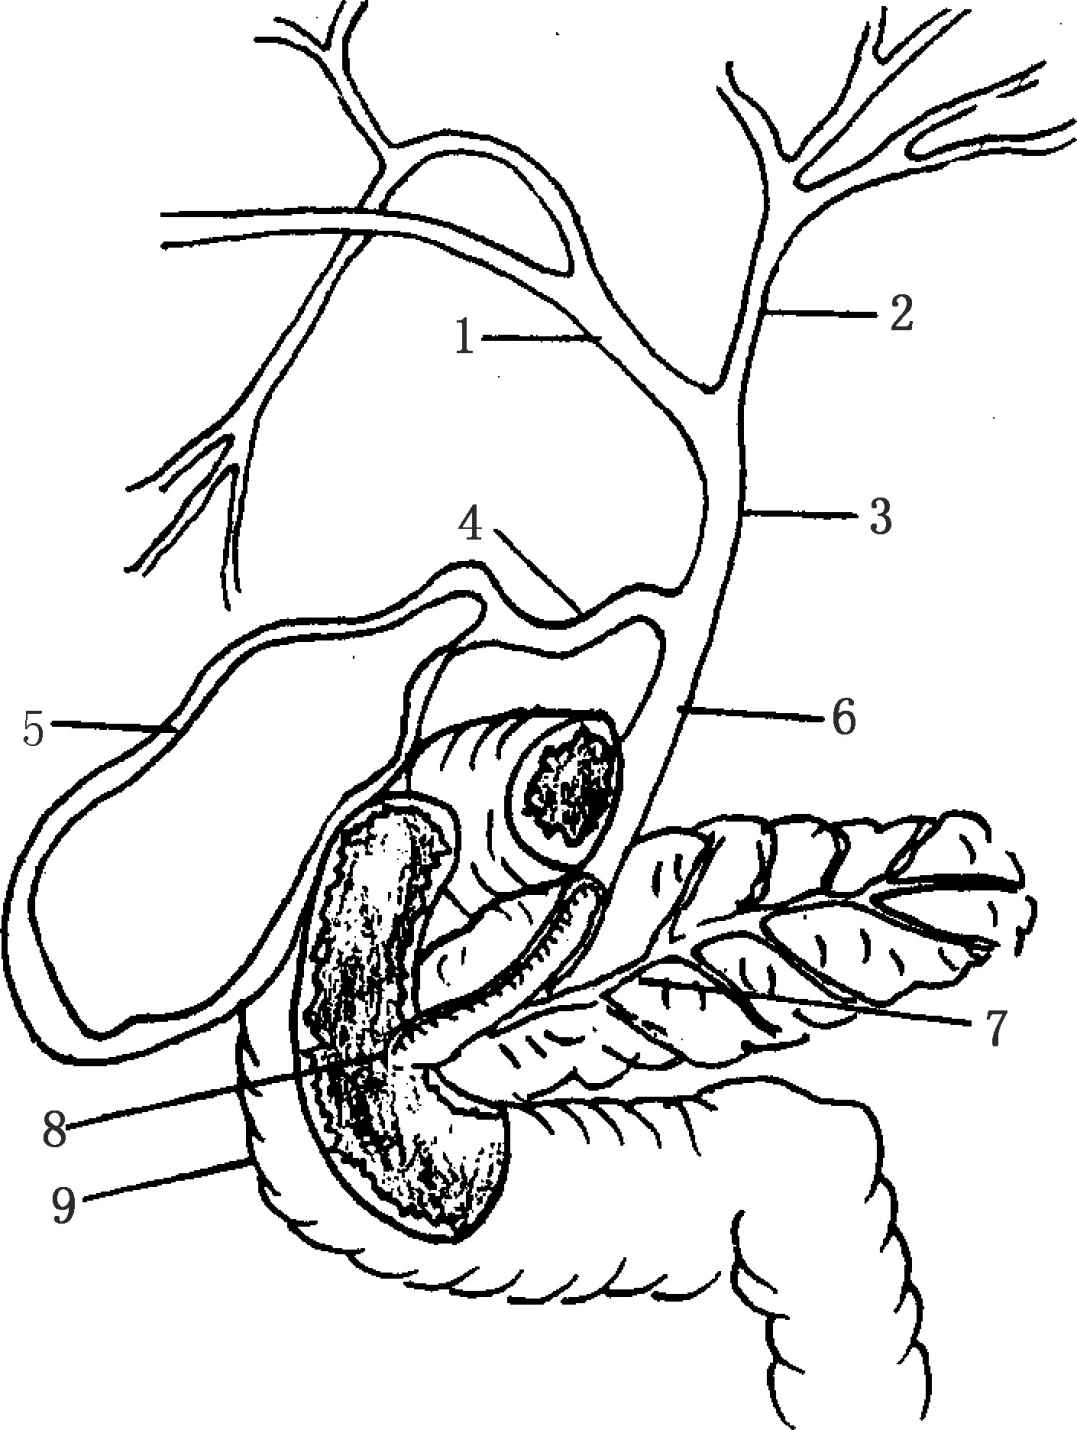
\includegraphics[width=.7\textwidth,height=\textheight,keepaspectratio]{./images/Image00290.jpg}
 \captionsetup{justification=centering}
 \caption{胆道系统解剖图\\{\small 1.右主肝管;2.左主肝管;3.肝总管;4.胆囊管;5.胆囊;6.肝总管;7.胰管;8.Vater壶腹;9.十二指肠降部}}
 \label{fig12-1}
  \end{figure} 

1.肝内胆管和肝总管:肝内毛细胆管逐渐汇合成小叶间、肝段、肝叶和左、右肝管,左、右肝管汇合成肝总管。在肝内,胆管、门静脉和肝动脉三者伴行。肝内胆管分支直径<2~3mm,或小于伴行门静脉的1/3,分辨率较差的CT不能显示,但在分辨率高的增强图上,少部分可以显示。通常只有很少一部分可见近肝门区肝内胆管,并呈散在分布,与梗阻所致的广泛扩张不同。

2.胆囊管:多在距十二指肠上缘2.5cm处与肝总管汇合成胆总管。

3.胆总管:分为4段。①十二指肠上段;②十二指肠后段;③胰腺段;④十二指肠壁内段。约82%的人可见其正常胆总管影。其长度差异大,少数胆囊管与肝总管汇合的位置很低,以致其上段不存在。80%与胰管汇合成乏特氏壶腹,其余则单独开口。胆总管出口的口径约为0.2cm,有奥狄氏括约肌环绕。胆总管直径多<6mm,6~10mm者为可疑扩张,>10mm者为扩张。

在肝门水平,肝总管与肝动脉并列位于门静脉的右前方、肝动脉的右侧,三者在横断面上呈三角形关系。胆总管大多数(80%)位于下腔静脉的正前方,胆总管与下腔静脉间距<10mm。

4.胆囊:为一倒置的梨形囊状器官,可分为3型,即圆形、梨形和长形。又分为底、体、漏斗和颈部,位于左叶内段与肝右叶前段之间的胆囊窝内。其内容物CT值为-5~20Hu。其横径>5cm提示增大,壁厚>3mm提示增厚。

正常胆道系统的有关径线见表\ref{tab12-1}。

\begin{table}[htbp]
\centering
\caption{胆道系统的径线}
\label{tab12-1}
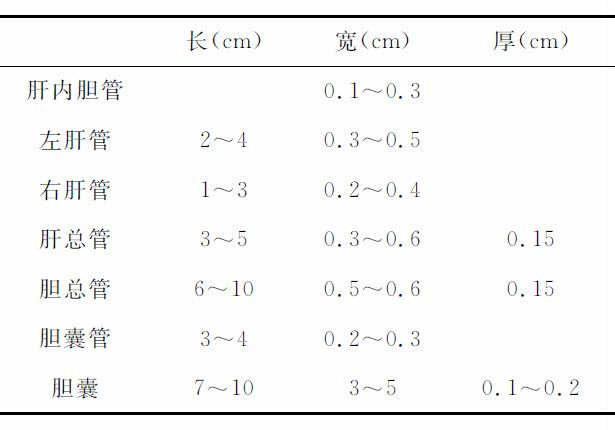
\includegraphics[width=\textwidth,height=\textheight,keepaspectratio]{./images/Image00291.jpg}
\end{table}

\subsection{胆囊和肝外胆管的先天性变异}

\subsubsection{胆囊的先天性变异}

①数目变异:胆囊缺如、双胆囊、三胆囊、胆囊闭锁;②体积变异:巨大胆囊、小胆囊;③形态变异:双房胆囊、叉状胆囊、葫芦状胆囊、三节胆囊、皱褶胆囊、扁平帽状胆囊及胆囊憩室;④位置变异:胆囊可位于肝右叶或肝左叶下方,以及肝后方(肝后胆囊常伴肝右叶萎缩或体积缩小);亦可埋于肝组织内(此型因胆囊收缩功能差,易感染并发结石);少数可呈游离胆囊(亦称漂浮性胆囊),是因胆囊支持韧带松弛,使胆囊呈游走状,多见于老年体瘦者,易发生扭转或通过网膜孔疝入小网膜囊内。

\subsubsection{肝外胆管的先天性变异}

①数目变异:副肝管、副胆囊管;②位置变异;③形态变异:先天性胆管狭窄或发育不良、先天性胆总管囊状扩张症。

\subsection{先天性胆管扩张症}

本病又称先天性胆管囊肿等。本病实际为先天性胆管的一部分囊状扩张。

\textbf{【发病机理】}
①胆管上皮增殖学说;②胰胆管合流异常学说:由于高浓度的胰液长期破坏胆管壁,引起炎性反应并逐渐扩张;③神经发育异常学说:类似先天性巨结肠改变,局部囊肿壁有神经节细胞缺陷。

\textbf{【病理】}
根据囊肿的形态、部位、范围等分为5型。Ⅰ型:最多见,约占80%~90%。为胆总管呈囊状或梭形扩张,胆囊及胆囊管多无明显异常。Ⅱ型:此型少见。为胆总管单发性憩室,多发生于胆总管之外侧壁,憩室蒂与胆总管可相通或闭塞不通。Ⅲ型:也少见。为胆总管下端十二指肠壁内段囊状扩张。Ⅳ型:较多见,约占18.9%。为多发囊状扩张,即肝内、肝外段多发囊状扩张,或肝外段多发囊状扩张。Ⅴ型:又称Caroli病(卡罗里病),属先天性常染色体隐性遗传病。为单发或多发的肝内胆管扩张,无肝外胆管扩张,即先天性肝内胆管扩张。其中Caroli病Ⅰ型多伴有结石和胆管炎,无肝硬化及门静脉高压;Caroli病Ⅱ型非常少见,伴有肝硬化及门静脉高压,不伴结石和胆管炎。Caroli病两型均可伴肾小管扩张,重者形成海绵肾。

\textbf{【临床表现】}
①先天性肝外胆管扩张:多见于10岁以下儿童,也可见于青年人,女性约为男性的3~4倍。黄疸、腹块及腹痛为本病的三大特征,但不一定同时出现。梗阻性黄疸多为间歇性,也可持续存在。②先天性肝内胆管扩张(Caroli病):主要表现为腹痛、肝大,也可有肝硬化和门静脉高压的症状和体征。③先天性肝内外混合型胆管扩张:兼有上述两种类型的特点。

\textbf{【CT表现】} 从影像学角度可分为下列3型。

1.肝外型:肝外胆管部分或全程囊样扩张,而肝内胆管不扩张(图\ref{fig12-2})。①囊肿位于肝门至胰头之间。②平扫或(和)增强扫描,囊肿均为圆形近水样低密度,不强化。囊壁可呈环形强化(厚约1~4mm),反复感染后壁较厚。囊肿大小不一,大者可达十几厘米。③胆囊及胆囊管多轻、中度扩张,但病程长者可缩小。④毗邻组织和器官受压、变形或移位,以胰头及十二指肠改变最具特点。⑤肝外多发胆管囊肿具有相应表现。

\begin{figure}[!htbp]
 \centering
 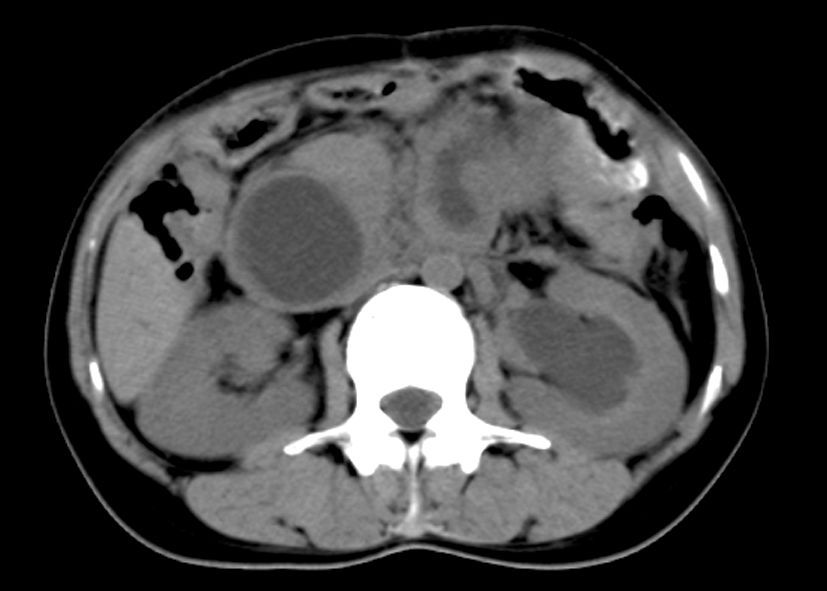
\includegraphics[width=.7\textwidth,height=\textheight,keepaspectratio]{./images/Image00292.jpg}
 \captionsetup{justification=centering}
 \caption{先天性胆管扩张症(肝外型)\\{\small 胆总管下端呈囊状显著扩张,左肾有积水表现}}
 \label{fig12-2}
  \end{figure} 

2.肝内型:即Caroli病。单独肝内胆管扩张,多见于远端肝内胆管,而肝外胆管不扩张。①肝内有多个囊状或柱状病变,呈水样密度,不强化。囊肿直径大小不一,大者可达4cm左右。②中心点征:异常扩张的胆管包绕相伴的门静脉小分支所致。③囊肿与柱状扩张的胆管相通,呈串珠状或分节状具有特征性,是与肝内非交通性囊肿的根本区别。④可合并胆管炎、胆石症、肝纤维化、肝硬化及门静脉高压、髓质海绵肾等。

3.肝内外混合型:即肝内外胆管同时扩张。其肝外改变同肝外型,而扩张的肝内胆管多为肝外扩张胆管向肝内的延续,主要累及近肝门区肝内胆管。肝内胆管扩张程度与胆总管扩张程度不成比例,有助于诊断。

\section{胆系结石、炎症和出血}

\subsection{胆系结石}

胆石症为胆道系统的最常见疾病,可发生在胆囊、肝内外胆管。

\textbf{【病因病理】}
其形成原因尚不完全明确,主要有以下几方面:①胆道感染;②胆道蛔虫;③代谢障碍;④神经功能紊乱和胆汁滞留。

胆系结石的化学成分主要为胆色素、胆固醇、钙质及其他少量的无机盐类。按化学成分可分为:①胆固醇结石:以胆固醇为主,其含量占80%左右,并含少量钙、蛋白及胆色素;②胆色素结石:此类结石在我国较多,呈砂粒状或桑椹状,可有少量钙盐和有机物质为核心;③混合类结石:是由胆色素、胆固醇和钙盐分层混合而成。

\textbf{【临床表现】}
与结石的位置、大小、胆道有无梗阻及并发症有关。多表现为右上腹不适及消化不良等症状;急性发作时,可有胆绞痛、呕吐、黄疸等;合并急性炎症时,出现高热等症状。

\textbf{【CT表现】}

\subsubsection{常见表现}

1.胆囊结石:①胆固醇结石:表现为单发或多发低密度及等密度结石,平扫多难以诊断,常需口服造影检查。②胆色素结石:表现为单发或多发的高密度灶,大小、形态各异(图\ref{fig12-3}A)。泥沙样结石沉积在胆囊下部呈高密度,与上部胆汁形成液平面。③混合性结石:表现为结石边缘呈环状高密度,中心为低密度或等密度(图\ref{fig12-3}B)。

2.肝外胆管结石:①胆管内圆形或环形致密影,近端胆管扩张(图\ref{fig12-3}B、C)。②结石位于胆管中心呈致密影,周围被低密度胆汁环绕,形成靶征;结石嵌顿于胆总管下端而紧靠一侧壁,则形成新月征或半月征。③胆总管扩张逐渐变细,且突然中断,未见结石和肿块,应考虑等密度结石可能。

3.肝内胆管结石:可局限于一叶或左、右叶均有,单发或多发,大小不等、形态各异。以管状、不规则状常见,亦可在胆管内形成铸型,并可见远侧胆管扩张。以高密度结石常见(图\ref{fig12-3}D)。

\begin{figure}[!htbp]
 \centering
 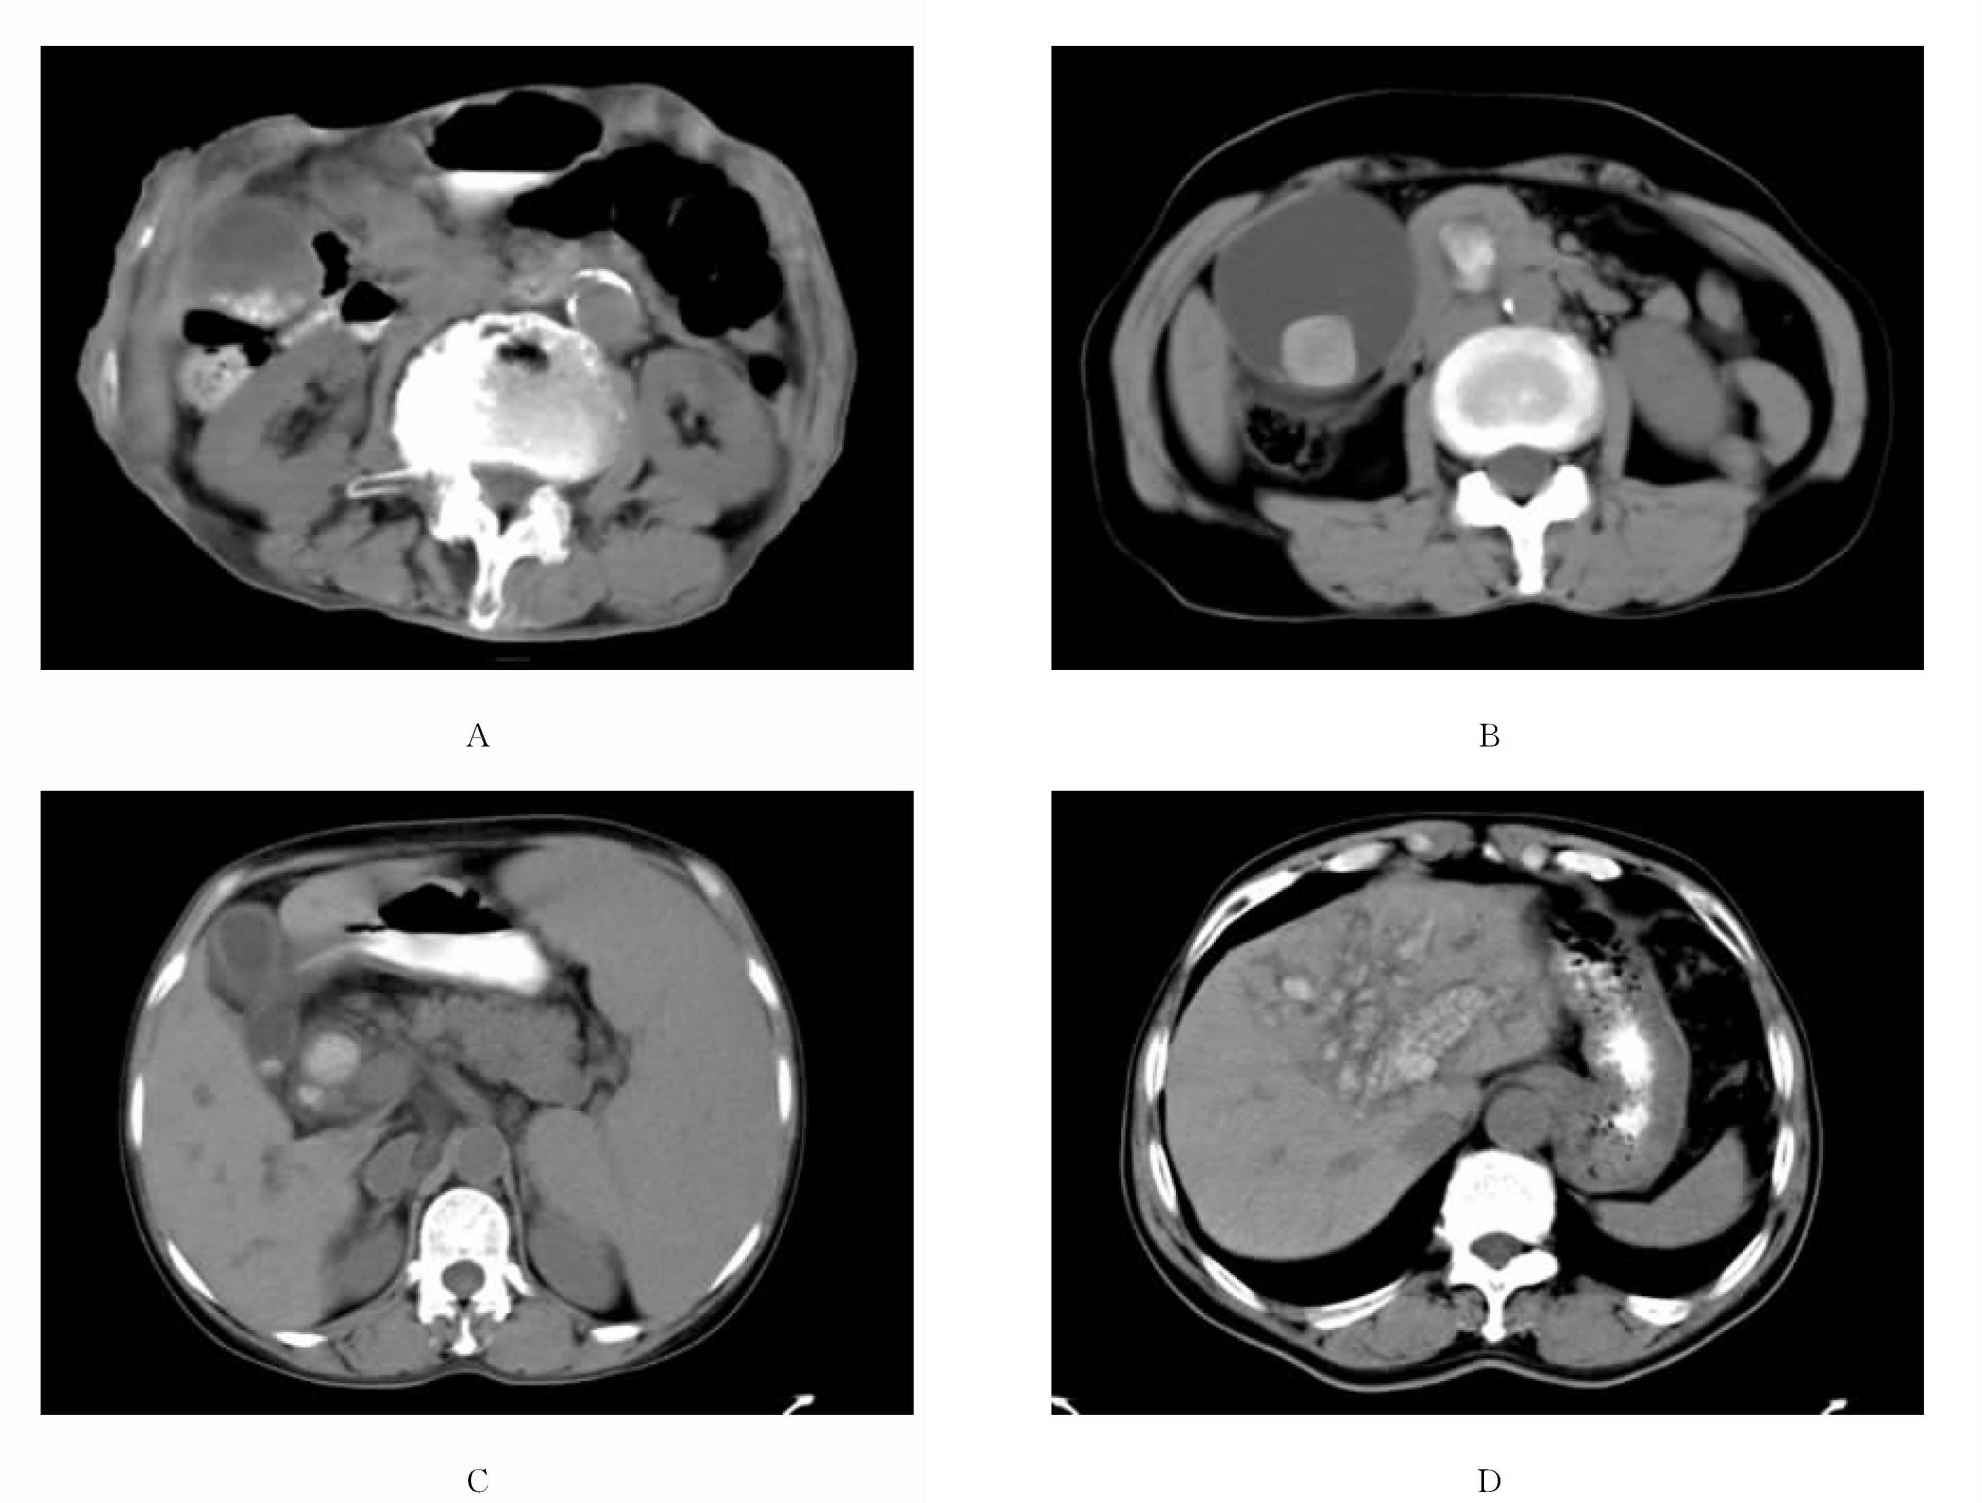
\includegraphics[width=.7\textwidth,height=\textheight,keepaspectratio]{./images/Image00293.jpg}
 \captionsetup{justification=centering}
 \caption{胆系结石\\{\small A.多发性胆囊结石;B.胆囊结石和胆总管结石;C.胆总管结石和胆囊颈部结石;D.多发性肝内胆管结石}}
 \label{fig12-3}
  \end{figure} 

但在诊断时应注意:①胆管结石排出后,胆总管因弹性减退或消失,不能恢复原状,可造成胆管梗阻的假象;肝内胆管周围受肝脏的保护,一般可恢复原状。②结石引起的梗阻常为不完全性或间歇性,其扩张可较轻或在临界范围内。

\subsubsection{结石成分的预测}

胆结石CT值与胆固醇含量呈负相关,与钙盐含量呈正相关。国外有学者对胆囊结石的体外研究认为:以CT值140Hu(范围135~145Hu)作为结石化学类型的预测阈值,其准确率达84%,即CT值<140Hu为胆固醇结石,>140Hu为混合性结石和胆色素结石。还有学者行鹅去氧胆酸溶石试验,结果结石CT值<50Hu或60Hu组大部分溶解,而>50Hu或60Hu组无一例溶解。

\subsubsection{CT分类}

国外有学者根据结石的CT表现,一般将结石分为以下几类。①高密度结石:CT值>90Hu者;②稍高密度结石:CT值26~67Hu;③环状高密度结石;④等密度结石:与盐水或胆汁相似;⑤分层状结石;⑥低密度结石。低密度、等密度、稍高密度结石以胆固醇性结石为主,其他则以非胆固醇性结石为主。

\subsubsection{钙胆汁}

胆汁中含有很高浓度的碳酸钙称为钙胆汁或石灰样胆汁。钙胆汁与胆结石有密切的关系。CT或X线表现为胆囊呈造影样高密度,在胆囊管区或胆囊内可见结石。有时可见胆汁分层。

\subsection{急性胆囊炎}

\textbf{【病因病理】}
本病多由结石嵌顿于胆囊颈部、胆囊管或细菌感染所致。病理可分为4类:①急性单纯性胆囊炎:胆囊黏膜充血、水肿、炎性细胞浸润。②急性化脓性胆囊炎:炎症波及胆囊壁全层,胆囊壁水肿、增厚,浆膜面纤维素渗出,胆囊内充满脓液。③急性坏疽性胆囊炎:胆囊壁缺血坏死及出血,胆囊内充满脓液,并可穿孔。④气肿性胆囊炎:由产气杆菌(多为梭状芽胞杆菌、产气荚膜杆菌,其次为大肠杆菌等)感染所致,胆囊内及其周围可见气体产生;30%发生于糖尿病患者,50%不存在结石。

\textbf{【临床表现】}
主要为急性右上腹痛,向肩胛区放射。多伴有高热、寒颤、恶心、呕吐、轻度黄疸。既往有胆绞痛发作史。莫菲氏征阳性。

\textbf{【CT表现】}
胆囊增大,为最常见的征象。胆囊壁弥漫性增厚为胆囊炎的重要依据,但不具特异性。增强扫描胆囊壁明显强化,且持续时间长。胆囊周围可见一周低密度环即“晕圈”征,为胆囊周围水肿所致(图\ref{fig12-4})。该征是胆囊炎,特别是急性胆囊炎的特征性征象。出血、坏死性胆囊炎时,胆囊内胆汁CT值升高。胆囊内或周围脓肿形成时,可见气体征象。有时可见胆囊扩张积液征象。气肿性胆囊炎可见胆囊壁内有气泡或线状气体,胆囊腔、胆道内及胆囊周围也可有低密度气泡影。

\begin{figure}[!htbp]
 \centering
 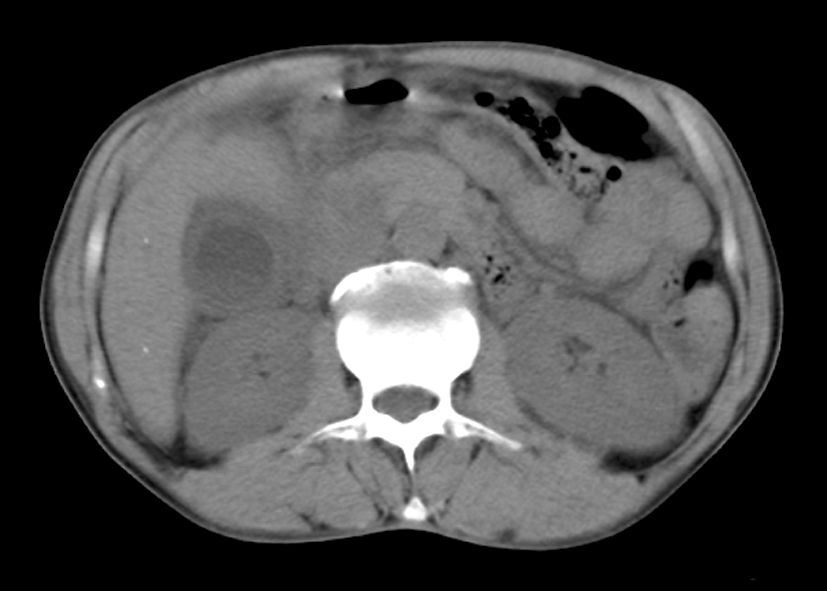
\includegraphics[width=.7\textwidth,height=\textheight,keepaspectratio]{./images/Image00294.jpg}
 \captionsetup{justification=centering}
 \caption{急性胆囊炎\\{\small 胆囊壁增厚,周围有水肿}}
 \label{fig12-4}
  \end{figure} 

此外,黄色肉芽肿性胆囊炎囊壁可高度不规则增厚,偶有钙化,容易穿孔并在肝内形成脓肿和肉芽肿,不易与胆囊癌鉴别。但是,黄色肉芽肿性胆囊炎增厚的囊壁内有大小不一、数目不等的圆形或类圆形低密度灶(主要由胆固醇、脂质及巨噬细胞构成),增强扫描无强化,是其特异性表现。

\subsection{慢性胆囊炎}

\textbf{【病因病理】}
本病为常见的胆囊疾病,可因细菌感染、化学刺激、乏特壶腹的炎症和肥厚等引起胆汁淤滞,以及代谢异常等所致。病理上胆囊黏膜萎缩、破坏;胆囊壁纤维化增厚,并可钙化;胆囊浓缩及收缩功能受损;胆囊可萎缩变小,亦可积水增大。

\textbf{【临床表现】}
主要为右上腹痛及反复发作性急性胆囊炎。其他有上腹不适、消化不良、饱胀等一般性症状。

\textbf{【CT表现】}
胆囊壁增厚为主要表现之一,增厚多较规则(图\ref{fig12-5})。一般认为胆囊扩张良好时,壁厚度≥3mm有诊断意义。胆囊壁钙化为特征性表现,如囊壁完全钙化称为“瓷胆囊”。胆囊可缩小或扩大,常合并胆囊结石。

\begin{figure}[!htbp]
 \centering
 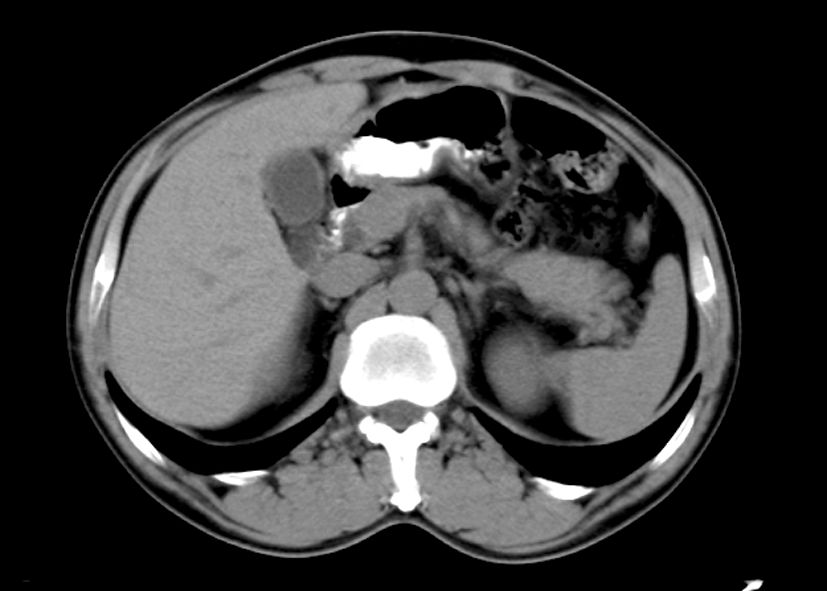
\includegraphics[width=.7\textwidth,height=\textheight,keepaspectratio]{./images/Image00295.jpg}
 \captionsetup{justification=centering}
 \caption{慢性胆囊炎\\{\small 胆囊壁增厚、密度增高,周围无水肿}}
 \label{fig12-5}
  \end{figure} 

\subsection{急性化脓性胆管炎}

\textbf{【病因病理】}
本病因胆管梗阻及感染引起,多见于胆管结石、胆道蛔虫,其次有胆管狭窄、肿瘤以及胰腺病变等。梗阻多位于胆总管下端。病理表现胆总管明显扩张,其内充满脓性胆汁,管壁炎性增厚,肝内可见多发脓肿。左肝管易使胆汁引流不畅、结石不易排出,而容易或加重感染,且感染可致肝实质萎缩。此外,所谓的复发性化脓性胆管炎是感染性胆管炎的反复发作,最终导致胆管狭窄、胆管梗阻和胆管结石。

\textbf{【临床表现】}
起病急骤,右上腹剧痛、高热、寒颤,多数有黄疸,甚至昏迷及死亡。复发性化脓性胆管炎患者可出现反复发作的腹痛、脓毒症和黄疸。

\textbf{【CT表现】}
肝内外胆管均明显扩张,其内充满脓汁,CT值高于胆汁。肝内胆管扩张常呈不对称性或局限分布,以左叶为著,扩张的胆管呈聚集状,是因左肝管易使胆汁引流不畅、结石不易排出所致。同时,扩张的胆管常局限在一、二级分支,而周围胆管因炎性纤维增生丧失扩张能力,表现为“中央箭头征”。胆管壁弥漫性增厚,其增厚可呈弥漫偏心性,增强扫描多于急性发作期呈明显强化。胆管内有时可见积气表现,常伴有胆管内结石。肝内可有多发性小脓肿。由于反复炎性阻塞、破坏,可有肝体积缩小或局限性萎缩,以左肝多见。

复发性化脓性胆管炎的基础疾病是肝内外胆管不规则扩张、胆系结石、胆囊炎、胆汁性肝硬化,典型的影像学表现是肝内胆管多房性囊性扩张并周边渐进性强化为特征(MR平扫、增强和MRCP对本病的诊断具有重要意义)。

\subsection{慢性胆管炎}

本病常由急性胆管炎发展而来。

\textbf{【病理】}
胆总管下端纤维瘢痕组织增生及狭窄,胆总管明显扩张,管壁增厚。

\textbf{【临床表现】}
中上腹不适、腹胀。急性发作时与急性化脓性胆管炎相同,可有高热、寒颤、黄疸三联征。

\textbf{【CT表现】}
①肝内、外胆管明显扩张,内有多发结石,是其常见和主要的CT表现。结石密度从等密度到高密度不等。结石的形态多种多样。肝内大的胆管扩张,而分支不扩张或扩张不明显。②肝外胆管壁呈广泛性、不规则增厚,壁厚可达2~3mm。

\subsection{原发性硬化性胆管炎}

本病又称狭窄性胆管炎,其病因不明,是一种罕见的慢性胆管阻塞性疾病。

\textbf{【病理】}
以肝内、外胆管的慢性进行性炎症及纤维化,最终导致胆管的短段狭窄与扩张交替为特征的病变。80%的病变累及包括胆囊在内的整个胆系,20%仅局限于肝外胆道。受累的胆管壁增厚、管腔狭窄,外径变化不大,内径明显缩小或闭塞。后期可发生胆汁性肝硬化或门静脉高压,9%~15%合并胆管癌。

\textbf{【临床表现】}
好发于40岁左右,男女之比约为2∶1。以慢性进行性黄疸为主要表现,一般无上腹绞痛史。合并肝硬化、门脉高压等并发症可有相应表现。87%伴发溃疡性结肠炎,13%伴发Crohn病。

\textbf{【CT表现】}
其主要CT征象为跳跃性扩张、串珠征和剪枝征。①病变局限于肝外胆管者,呈典型的低位梗阻表现,狭窄处远端的胆总管仍可见。狭窄处胆管壁增厚,管腔狭小,密度增高;增强扫描管壁强化明显。可有或无胆囊壁增厚。如某段扩张的肝外胆管不与其他扩张的胆管相连称为“跳跃性扩张”,其形成基础是肝内胆管狭窄合并远段胆管扩张。②病变广泛者呈不连续的散在分布的串珠状或不规则状,反映了其多发性狭窄。段性分布的肝内胆管扩张也是其表现之一。在1个层面上见到3处以上狭窄与扩张交替出现,称为“串珠征”。但此征也可见于恶性病变。③剪枝征:即某1层面上见到长度≥4cm的肝内胆管或左右肝管,而无次级分支称为“剪枝征”。本病25%的可见此征,但13%~15%的恶性病变也可见此征。④晚期可见肝硬化、门脉高压表现,还可见大量的肝内胆管钙化影。

通常本病引起的肝内胆管扩张程度较轻,有明显扩张者要想到肿瘤性病变。

\textbf{【鉴别诊断】}
应注意结合病史与结石、胆系感染和手术等原因所致的继发性硬化性胆管炎相鉴别。

\subsection{胆道出血}

胆道出血是肝胆疾病的严重并发症。

\textbf{【病因】}
其病因很多,主要有肝内感染、肝内胆管结石、手术时的探查和肝损伤等。

\textbf{【临床表现】}
临床有不明原因的消化道出血。DSA有助于进一步确诊,并指导介入治疗。

\textbf{【CT表现】}
血液通过开放的胆总管进入胆囊,当出血量占胆囊容量的70%和出现血凝块时,表现为胆囊不均匀性密度增高。出血量更大时,胆囊内密度均匀性增加,CT值高达50~60Hu。胆系出血常合并胆道梗阻,引起扩张、积血,表现为胆管扩张,其内见管状或圆形高密度灶。

本病需注意与钙胆汁(其密度高于出血15~20Hu)、胆管结石相鉴别。结合临床对本病的诊断和鉴别有重要作用。

\section{胆囊息肉样病变}

\subsection{胆囊胆固醇沉着症}

本病是因胆固醇代谢障碍沉积于胆囊壁,在黏膜表面形成黄色小赘生物。

\textbf{【病理】}
根据其形态分为:①扁平型:病变广泛,黏膜增厚,表面粗糙,有多个类似绒毛状或草莓状小隆起;②息肉型:病变局限,多为单发或多发息肉样隆起,称为胆固醇息肉;大小多<1cm,有蒂或无蒂。

\textbf{【临床表现】}
一般无明显症状,合并胆石、慢性胆囊炎时可有相应临床症状。

\textbf{【CT表现】}
与胆囊炎性息肉形态无法区别。可为桑椹状,有蒂或无蒂,多为多发,大小多<5~6mm。一般CT检查难以发现,胆囊造影CT检查有助于病变的检出。

\subsection{胆囊腺瘤和炎性息肉}

胆囊腺瘤和炎性息肉病理是截然不同的两个疾病,但CT表现相似。

\textbf{【病理】}
胆囊腺瘤一般为单发,表面较光滑,也可不规则如小菜花状;多发生在体部,靠近底部;一般比炎性息肉稍大。炎性息肉为增生的纤维结缔组织,伴有淋巴及单核细胞等炎性细胞浸润,表面被覆增生的上皮;单发或多发,多位于胆囊底部,形态不规则,可有蒂。

\textbf{【临床表现】} 一般无明显症状,合并胆囊炎时可有相应临床症状。

\textbf{【CT表现】}
两者CT表现基本相同,普通CT检查难以发现。①薄层CT扫描有时可见小结节状病灶由胆囊壁突向腔内,CT值介于胆固醇结石与胆色素结石之间。②胆囊炎性息肉常多发,直径多在0.4~0.6cm;胆囊腺瘤常单发,直径0.5~4.0cm,表面相对较光滑。③口服胆囊造影可显示胆囊内充盈缺损,变换体位病灶位置固定有别于等密度或低密度结石。

\textbf{【鉴别诊断】}
两者均无胆囊壁浸润增厚有别胆囊癌,但与早期胆囊癌难以鉴别,一般认为息肉和腺瘤直径>1cm者有恶性变可能。

\subsection{胆囊腺肌增生症}

本病命名有20余种,国内多称为胆囊腺肌增生症,国外多称为胆囊腺肌瘤病。本病比较常见,发病率为2.8%~5.0%。

\textbf{【病因病理】}
病因尚不十分明了,有人认为与感染和结石有关;目前多认为与胚胎期胆囊芽囊化不全有关;也有作者认为与胆囊动力学障碍,胆囊内压力增高使黏膜伸入黏膜下层和肌层而形成罗-阿(Rokitansky-Aschoff)窦有关。病理表现主要是胆囊黏膜和肌纤维增生肥厚,增生的黏膜伸入肌层(甚至达浆膜面)形成罗-阿氏窦。这些窦腔与胆囊腔相通,窦内可有胆汁淤积、胆固醇沉积或小结石形成。窦腔多<0.8cm,>2.0cm者少见。根据其病理改变、病变范围和影像学表现可分为3型:①弥漫型:侵及全部胆囊;②节段型:侵及胆囊体部或颈部的一节段;③局限型或基底型:此型多见,侵及胆囊底部的一部分,中心常可见一脐样凹陷。

\textbf{【临床表现】}
无特异性,少数无症状。一般病程较长,症状轻重不一。主要为消化不良、食欲减退及上腹饱胀,常有右上腹隐痛,尤以进脂肪餐时症状加重或产生胆绞痛。如伴有结石,类似胆囊炎、胆石症症状。还有报道患者出现不明原因的发热。

\textbf{【CT表现】}
主要表现为胆囊壁增厚,以及伸入壁内的且与胆囊腔相通的多个小壁内憩室;增厚的胆囊壁内有结石影亦是其特征之一。胆囊造影有助于确诊,脂肪餐后罗---阿氏窦内造影剂充盈更著,分布在充盈造影剂的胆囊腔边缘,类似花环状称为“花环征”,为其特异性表现。增强扫描动脉期增厚的胆囊壁均表现为黏膜层和黏膜下区强化;门静脉期强化扩展;延迟期胆囊壁强化范围进一步扩大,胆囊壁全层呈不均匀显著强化或较均匀强化,这种强化方式其他疾病少见(图\ref{fig12-6})。胆囊与肝脏界限清晰。

\begin{figure}[!htbp]
 \centering
 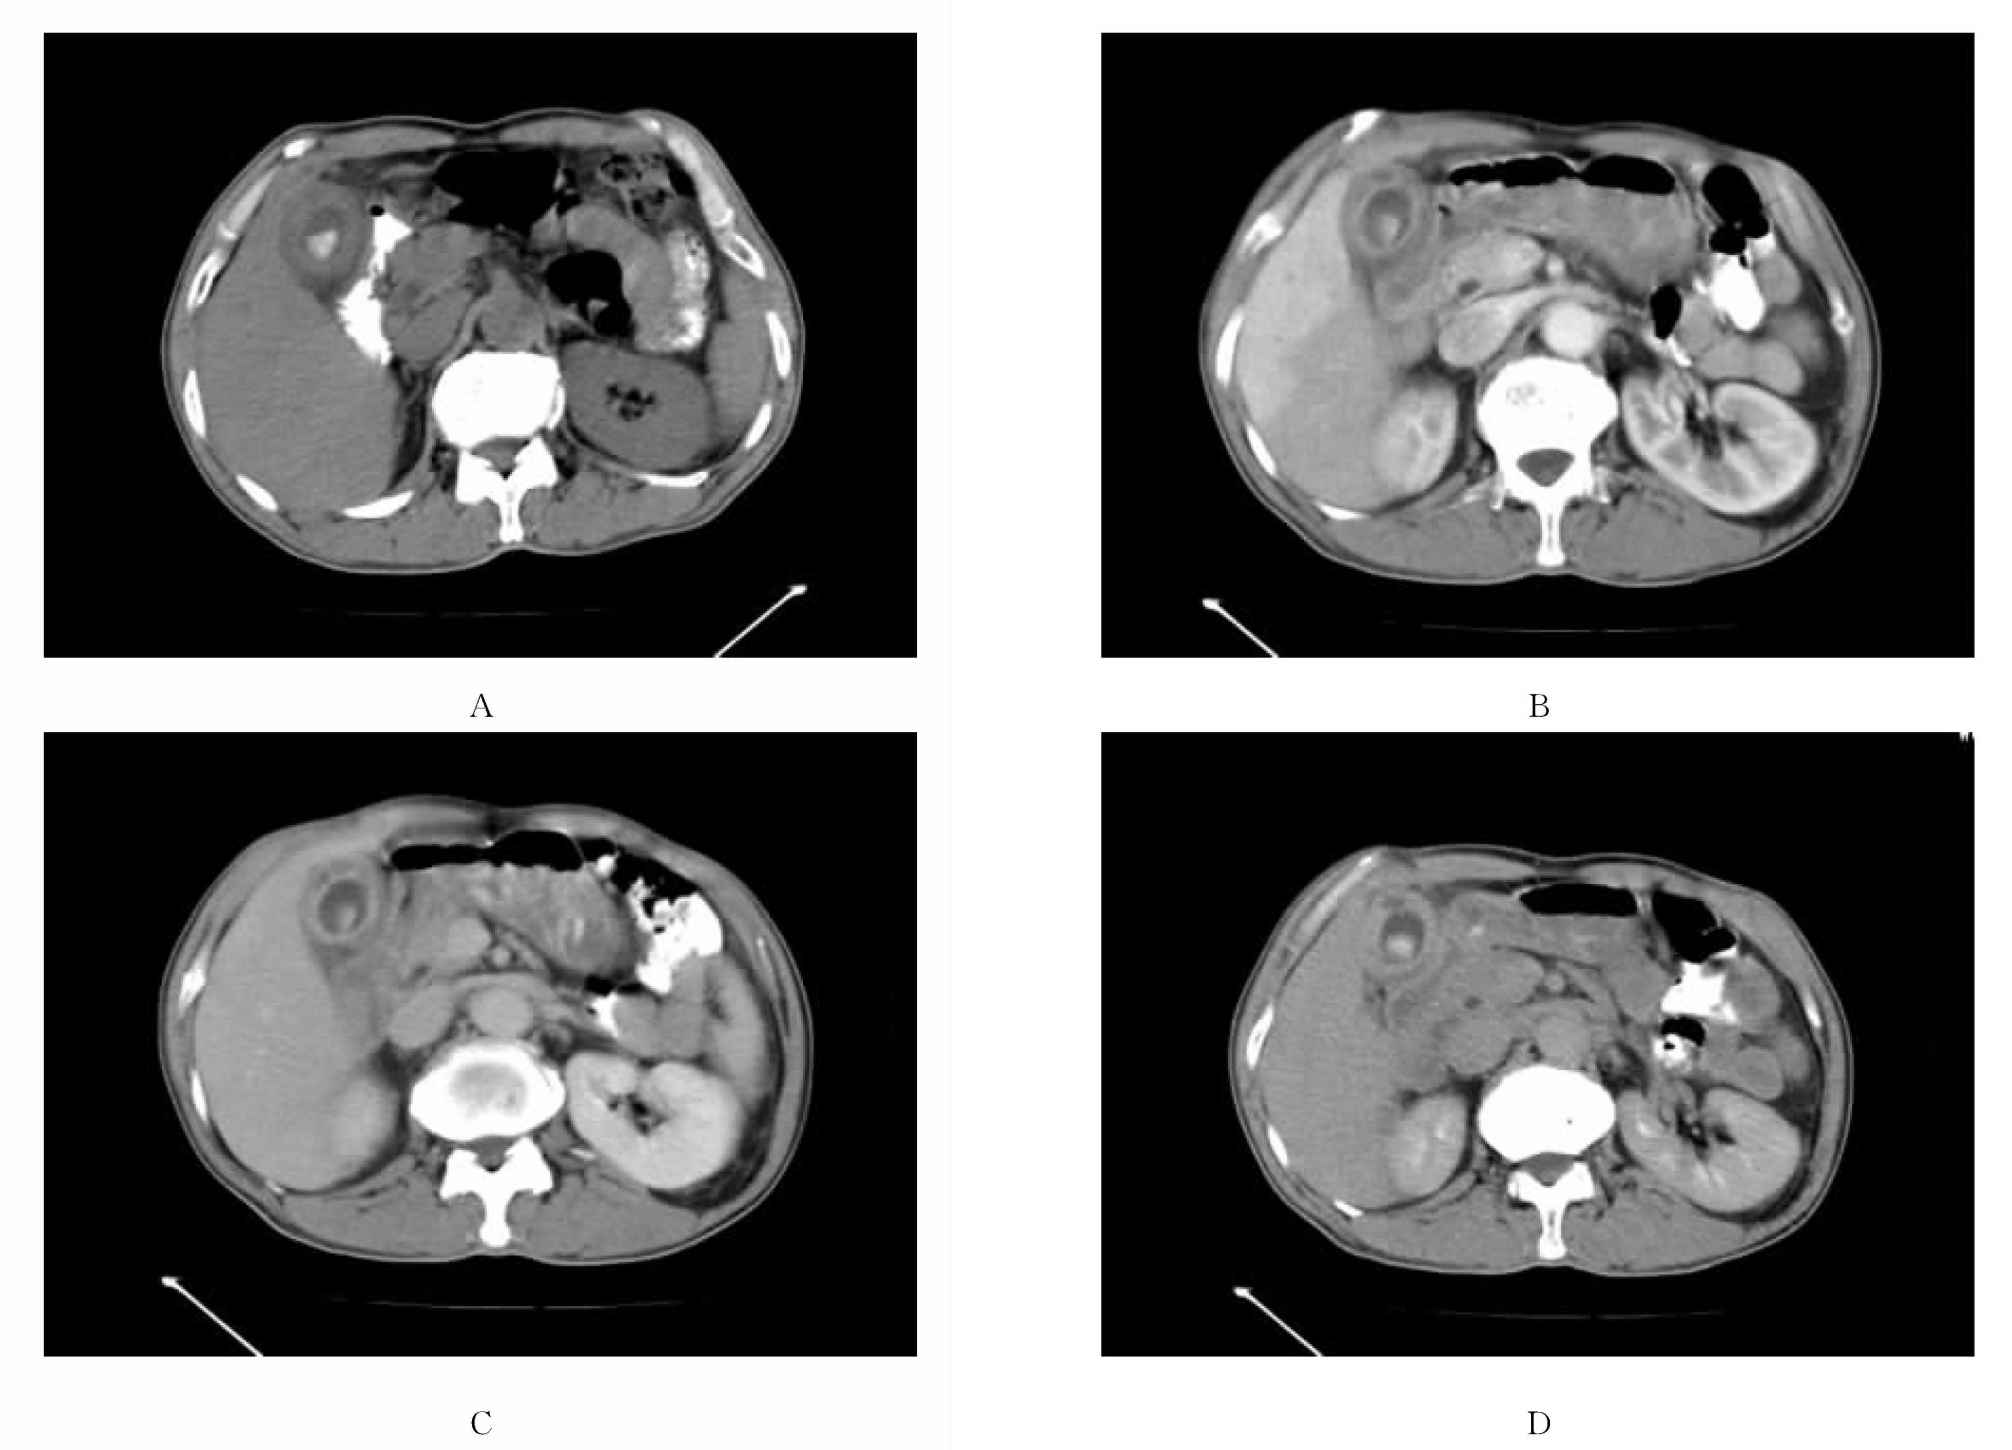
\includegraphics[width=.7\textwidth,height=\textheight,keepaspectratio]{./images/Image00296.jpg}
 \captionsetup{justification=centering}
 \caption{胆囊腺肌增生症\\{\small A~D为同一患者,A为平扫,B~D为增强扫描。A.胆囊壁弥漫性较均匀增厚,其内有高密度结石;B.动脉期增厚的胆囊壁均表现为黏膜层和黏膜下区强化;C.门静脉期强化范围扩展;D.延迟期胆囊壁全层呈较均匀强化,壁内有小囊状低密度灶。胆囊与肝脏界限清晰}}
 \label{fig12-6}
  \end{figure} 

分型:①弥漫型:表现为整个胆囊壁增厚;口服胆囊造影CT可见“花环征”或“光环征”。②节段型:表现为胆囊壁中部(体部、颈部)节段性肥厚,胆囊腔局限性狭窄;口服造影亦可显示“花环征”或“光环征”。③局限型或基底型:胆囊底部局限性增厚状如三角形小帽,国内有学者称为“小帽征”,高度提示本病;口服造影可见壁内小憩室样突出或底部中心可见脐样凹陷。

\subsection{胆囊息肉样病变的鉴别诊断}

1.好发部位:胆固醇息肉和炎性息肉好发于体部;腺肌增生症好发于底部;腺瘤好发于颈、体部;腺癌好发于颈、底部。

2.病变大小:腺肌增生症>腺癌>腺瘤>炎性息肉>胆固醇息肉。

3.病变数目:胆固醇息肉和炎性息肉易多发;腺肌增生症、腺瘤、腺癌常单发。

4.与胆囊壁的关系:胆固醇息肉基底窄,常有细蒂;炎性息肉基底窄无蒂;腺肌增生症基底宽无蒂,可见罗-阿氏窦;腺瘤基底较宽可有蒂;腺癌基底宽无蒂,常有局部胆囊壁浸润增厚。

对此类病变的显示以B超显示为优。超声还可见病灶内部回声的强弱为:腺肌增生症>胆固醇息肉>炎性息肉>腺瘤>腺癌。

\section{胆系恶性肿瘤及肝外胆管梗阻}

\subsection{胆囊癌}

胆囊癌占恶性肿瘤的0.3%~5%,是胆道最常见的恶性肿瘤,65%~90%合并胆囊结石和慢性胆囊炎。早期预后好,但诊断困难。

\textbf{【病因病理】}
病因不明,多认为与胆石症和慢性胆囊炎对胆囊黏膜的长期刺激导致黏膜上皮细胞的突变有关。病理组织学以腺癌最常见,占70%~90%,鳞癌占10%,其他如未分化癌、肉瘤和类癌等罕见。腺癌又分为:①浸润型:约占70%,早期局限性胆囊壁增厚,晚期形成肿块、囊腔闭塞;②乳头状型:约占20%,肿瘤呈乳头状或菜花状从胆囊壁突向腔内,肿瘤易坏死、溃烂出血和感染;③黏液型:约占8%,胆囊壁往往有广泛浸润,肿瘤呈胶状易溃破,甚至引起胆囊穿孔。

转移途径:主要有直接侵犯、淋巴转移、血行转移、胆管内转移及腹腔内种植等,其中以直接侵犯及淋巴转移为主,而血行转移不常见。

\textbf{【临床表现】}
以50岁以上女性多见,早期症状多系伴发结石所致,无特异性。后期有进行性体重减轻、恶液质及右上腹持续性疼痛,甚至出现黄疸、发热和腹水。半数病人右上腹可扪及肿块。

\textbf{【CT表现】}

1.直接征象:其CT表现常分为以下4型。①肿块型:胆囊腔大部分或完全消失,被实性软组织肿块代替,与肝实质密度相似,其分界不清。此型多为晚期表现,常合并胆道梗阻,少数难以区分来自肝脏还是胆囊。②壁厚型:胆囊壁局限性或弥漫性不规则增厚,内缘凹凸不平,外缘多毛糙,胆囊壁密度多不均匀。少数均匀增厚,类似慢性胆囊炎。③结节型:表现为从胆囊壁向腔内突出的乳头状或菜花状肿块,单发或多发。其基底部的胆囊壁多浸润增厚(图\ref{fig12-7})。④阻塞型:肿瘤侵犯胆囊管造成阻塞,胆囊积液增大,胆囊壁略增厚或不增厚。因肿瘤小往往不易发现,增强扫描有时可见小的肿瘤。此外,还有个别报道呈外生型生长。

增强扫描肿瘤强化显著,且持续时间长,强化多不均匀(图\ref{fig12-7});胆囊黏膜线多破坏残缺。

\begin{figure}[!htbp]
 \centering
 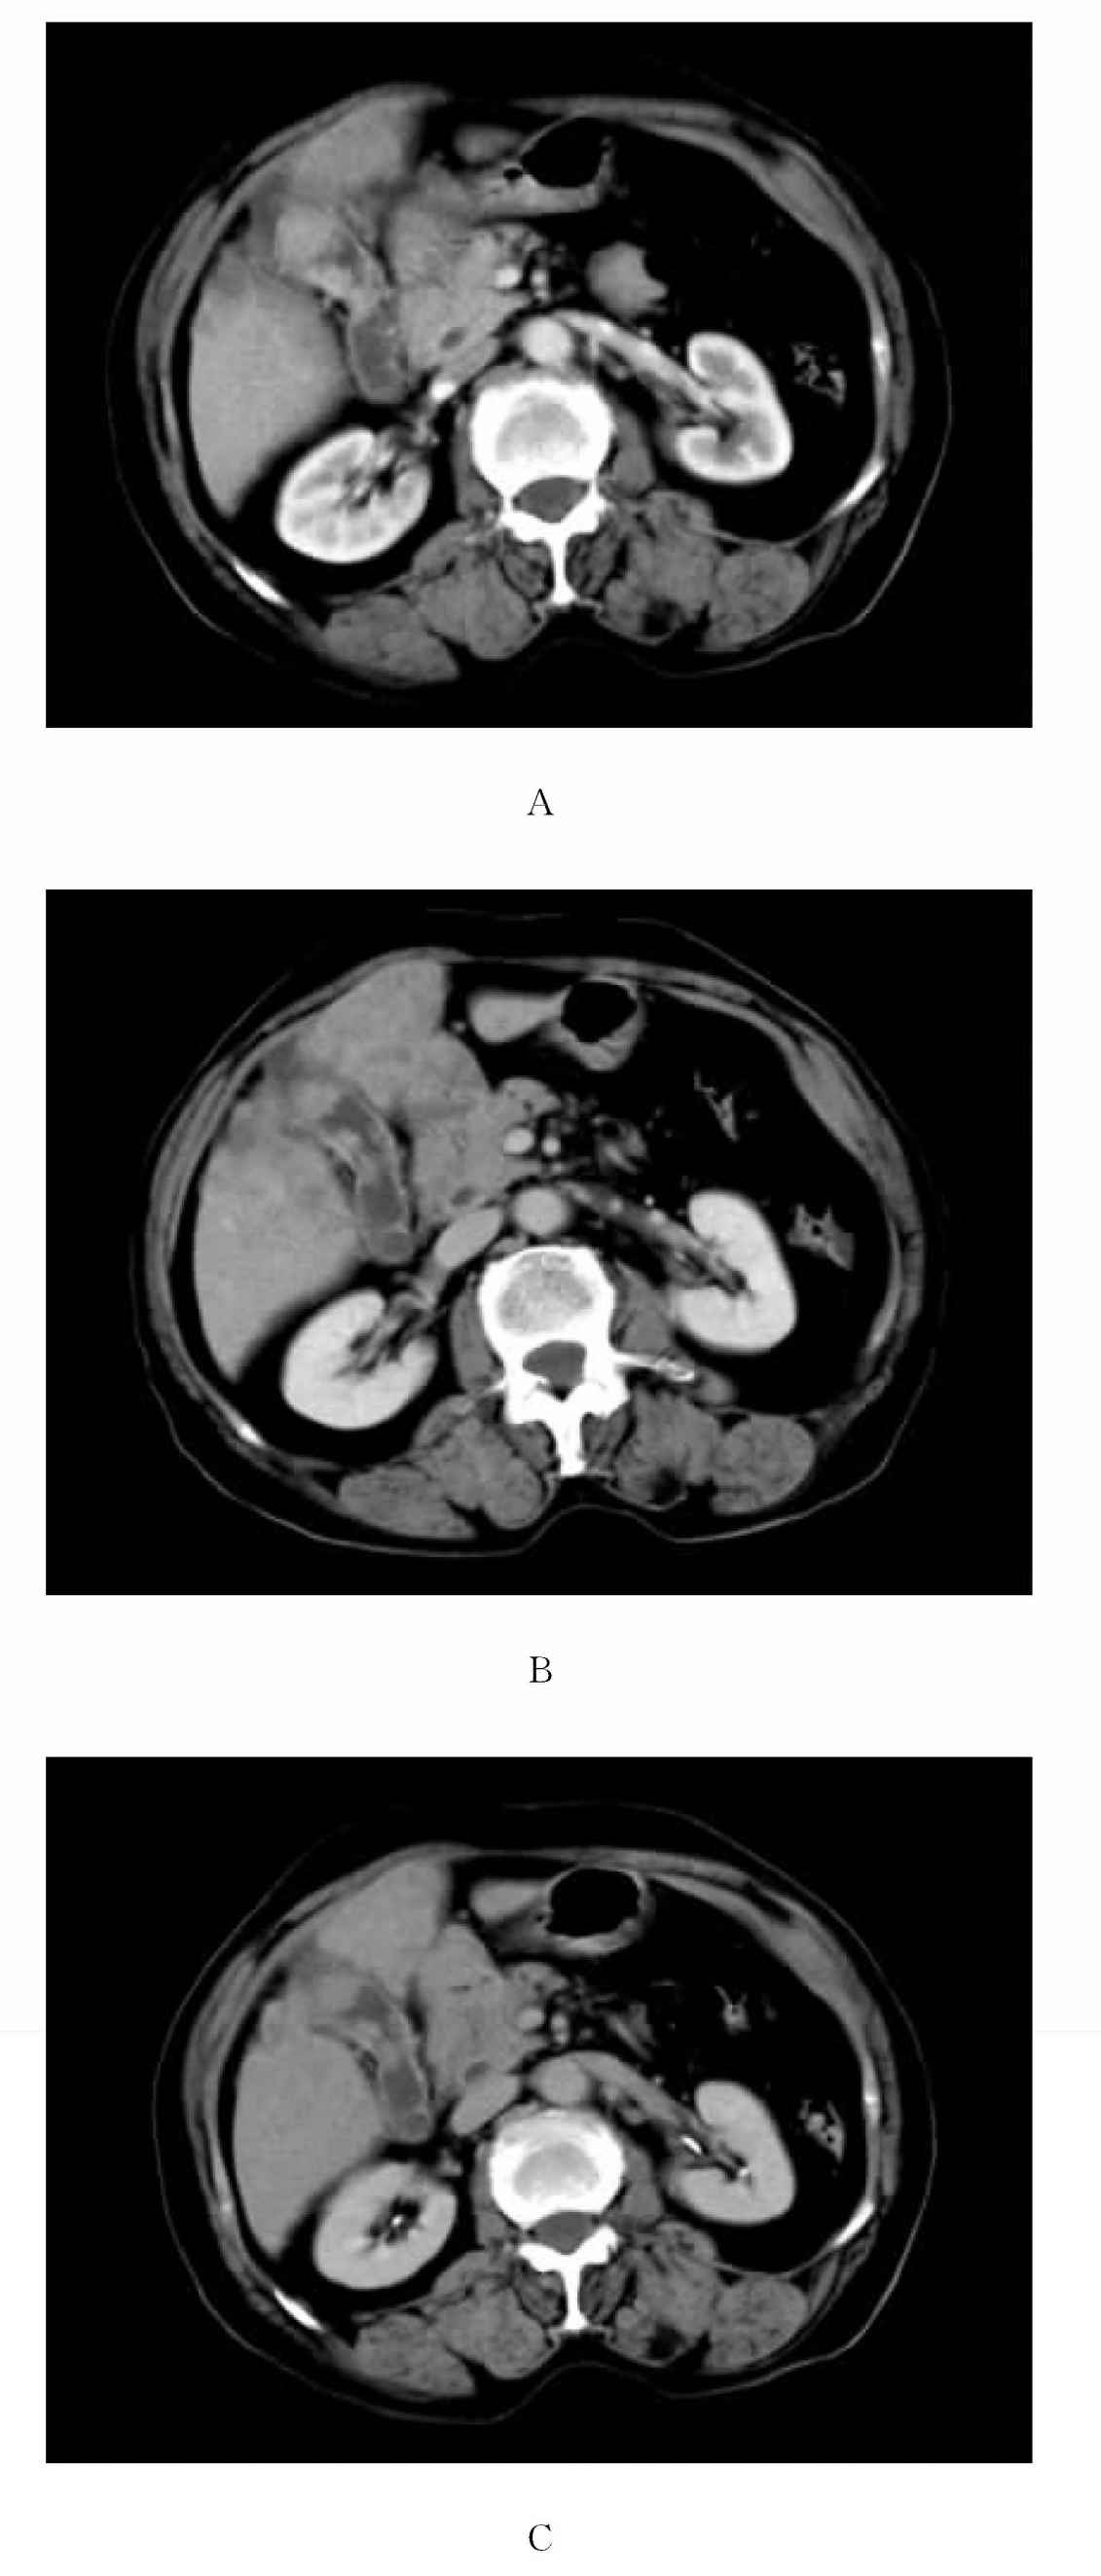
\includegraphics[width=.7\textwidth,height=\textheight,keepaspectratio]{./images/Image00297.jpg}
 \captionsetup{justification=centering}
 \caption{胆囊癌\\{\small A~C为同一患者的增强扫描。A为动脉期,B为门静脉期,C为平衡期;胆囊底、体部有多个高密度强化的结节,边缘不规则,胆囊底部的邻近肝脏受侵}}
 \label{fig12-7}
  \end{figure} 

2.间接征象:①肝脏直接受侵:表现为胆囊床界限模糊,肝组织呈不规则低密度;②肝内转移灶;③淋巴结转移;④胆道梗阻征象:侵犯胆囊管及肝总管或淋巴结转移压迫肝总管所致;⑤门静脉浸润征象:甚至可形成瘤栓,但不及肝癌常见;⑥相邻器官受侵:如胃窦、十二指肠、胰头受侵;⑦合并胆囊结石及慢性胆囊炎征象,故胆囊无功能、“瓷胆囊”、胆囊内充满结石等,应警惕胆囊癌可能;⑧腹水。

\textbf{【CT诊断标准】}
结合有关资料,我们认为以下几点可作为其CT诊断标准:①不均匀增强的团块状肿块或胆囊壁增厚>1cm,且伴有病灶扩散或周围受侵可确诊为胆囊癌。②病灶>1cm不伴有扩散或周围受侵为胆囊癌可能。③病灶≤1cm不伴有扩散或周围受侵,基本排除胆囊癌。

胆囊癌的CT诊断虽很有价值,但仍有其局限性:①胆囊壁的增厚既见于慢性胆囊炎,也见于胆囊癌,有时难以鉴别。②某些晚期病例CT难以区分占位是肝癌侵及胆囊,还是胆囊癌侵犯肝脏。③个别早期胆囊癌可以漏诊,尤其厚层扫描时。④胆囊癌所致的胰头周围淋巴结增大,可以酷似胰腺癌。⑤胆囊癌的肝内胆管和胆总管内播散常难以被发现,一些阳性发现者可误为胆管细胞癌。

\textbf{【鉴别诊断】}

1.肝癌:①胆囊癌伴胆管扩张的几率高于肝癌;②胆囊癌强化明显,且峰值持续时间长,与肝脏界限不清;而肝癌的强化呈速升速降型,且峰值持续时间短;③软组织肿块内见到结石影,支持胆囊癌的诊断;④当胆囊窝只有肿块而未见胆囊,应首先考虑胆囊癌,并进一步增强扫描。

2.胆囊炎:多数胆囊壁炎性增厚可见:①呈双边或多边征象;②均匀增强,腔内面光滑;③周围见渗出性改变,有时出现气体征象;④增强扫描黏膜线多无中断。而胆囊癌胆囊壁增厚多呈结节状、胆囊壁增强明显、厚壁型胆囊癌黏膜线多中断,易出现胆管梗阻,并直接侵及肝脏等有别于胆囊炎。但国内有关文献报道厚壁型胆囊癌与慢性胆囊炎、黄色肉芽肿性胆囊炎的影像学表现相似,难以鉴别。

3.胆囊腺肌增生症:口服或静脉胆囊造影所见的罗-阿氏窦有助于鉴别。增厚的胆囊壁内有少量钙化(小结石)或罗-阿氏窦则为胆囊腺肌增生症可能,如见明显的钙化(小结石)或罗-阿氏窦则确诊为胆囊腺肌增生症。此外,其动态增强的强化方式有一定特点。

此外,①胆囊壁钙化、胆汁高度浓缩时附着于囊壁类似肿块,或囊腔充满浓缩胆汁应与增强效果较差的胆囊癌鉴别。②小的腔内型胆囊癌应与息肉、腺瘤、胆囊乳头状瘤等鉴别,但可有困难。

\subsection{胆管癌}

本病在胆道恶性肿瘤中的发病率仅次于胆囊,居第二位。

\textbf{【病因病理】}

1.按位置通常分为3型:①肝内胆管癌:又称周围型胆管癌(见第十一章第四节);②肝门区胆管癌:指起源于肝总管分叉和左、右主肝管胆管上皮者,约占67%;③远段胆管癌。还有人将其分为肝内、肝外型,肝外型包括肝门型、肝外胆管型和壶腹型。

肝门区胆管癌近年来有上升趋势,其发病与慢性胆道感染、结石、溃疡性结肠炎、Caroli病、硬化性胆管炎、胆管内乳头状瘤、华支睾吸虫感染及钍放射线损伤等多种因素有关。

2.按病理形态通常分为3型:①肿块型;②管壁浸润型;③管内型。其中以管壁浸润型多见。

3.本病病理组织学多为中或低分化腺癌,其中硬癌占87%~94%,乳头状癌占6%~13%。罕见的有鳞状上皮癌、腺鳞癌。

\textbf{【临床表现】}
本病多发生于50~70岁,以男性多见。起病隐匿,发病初期右上腹和上腹胀痛。随着病情发展,出现梗阻性黄疸,且进行性加重。可伴有胆管炎的症状。

\textbf{【CT表现】}

1.肝门区胆管癌

其CT表现分类方法很多,常分为两类。①浸润型:表现为近左、右肝管汇合处肝管管壁局限性不规则增厚,管腔不同程度狭窄。增强后管壁可有强化(图\ref{fig12-8}),多有延迟强化的特点。②结节型:局部有低或略低软组织肿块伴肝管狭窄或中断,肿块可向腔内生长,亦可向腔外生长。增强后轻度强化,强化期出现在门静脉期或延迟期。



\begin{figure}[!htbp]
 \centering
 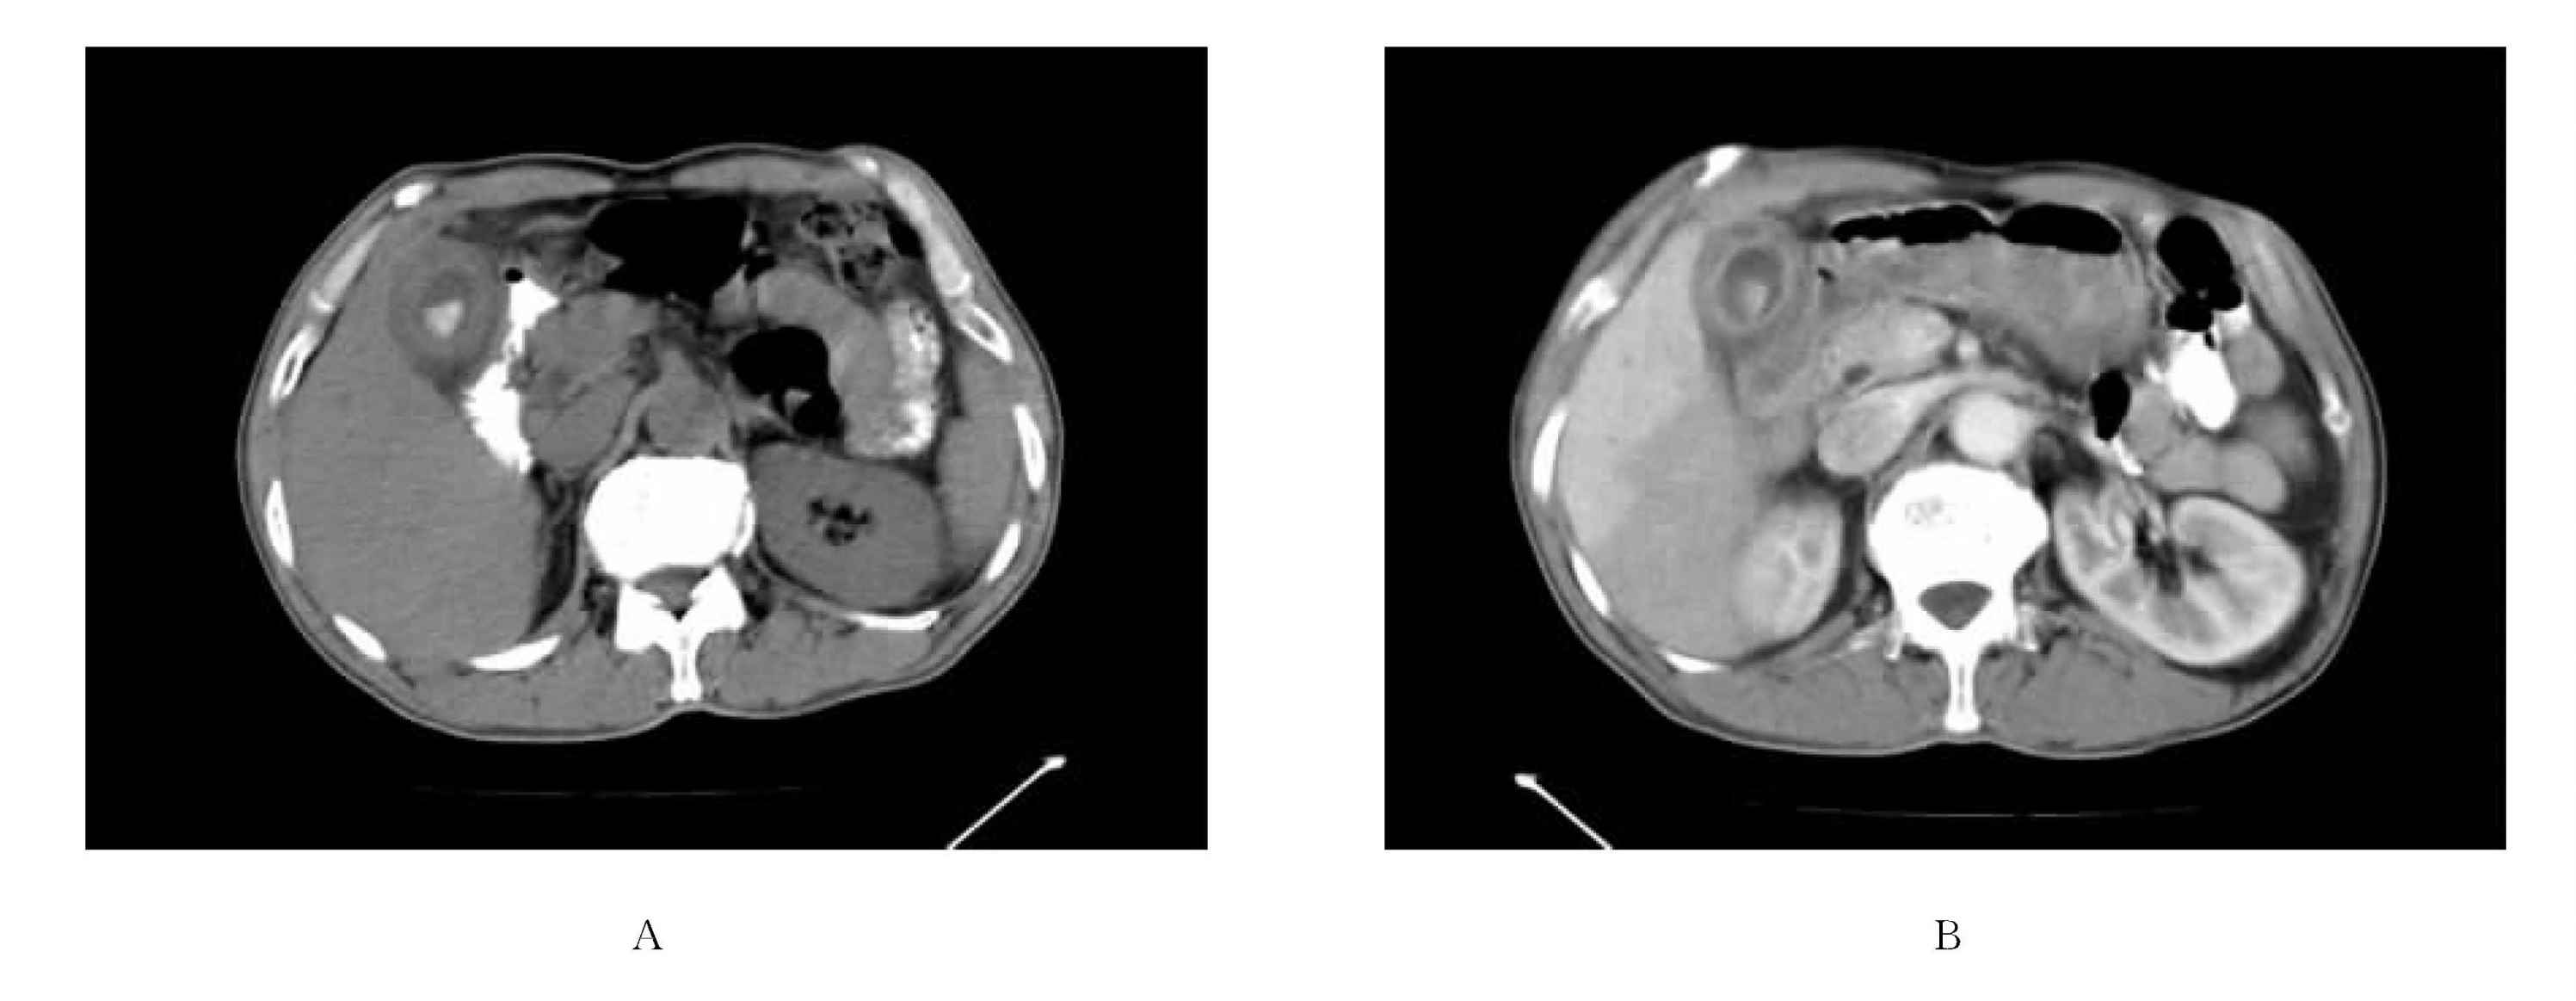
\includegraphics[width=.7\textwidth,height=\textheight,keepaspectratio]{./images/Image00298.jpg}
 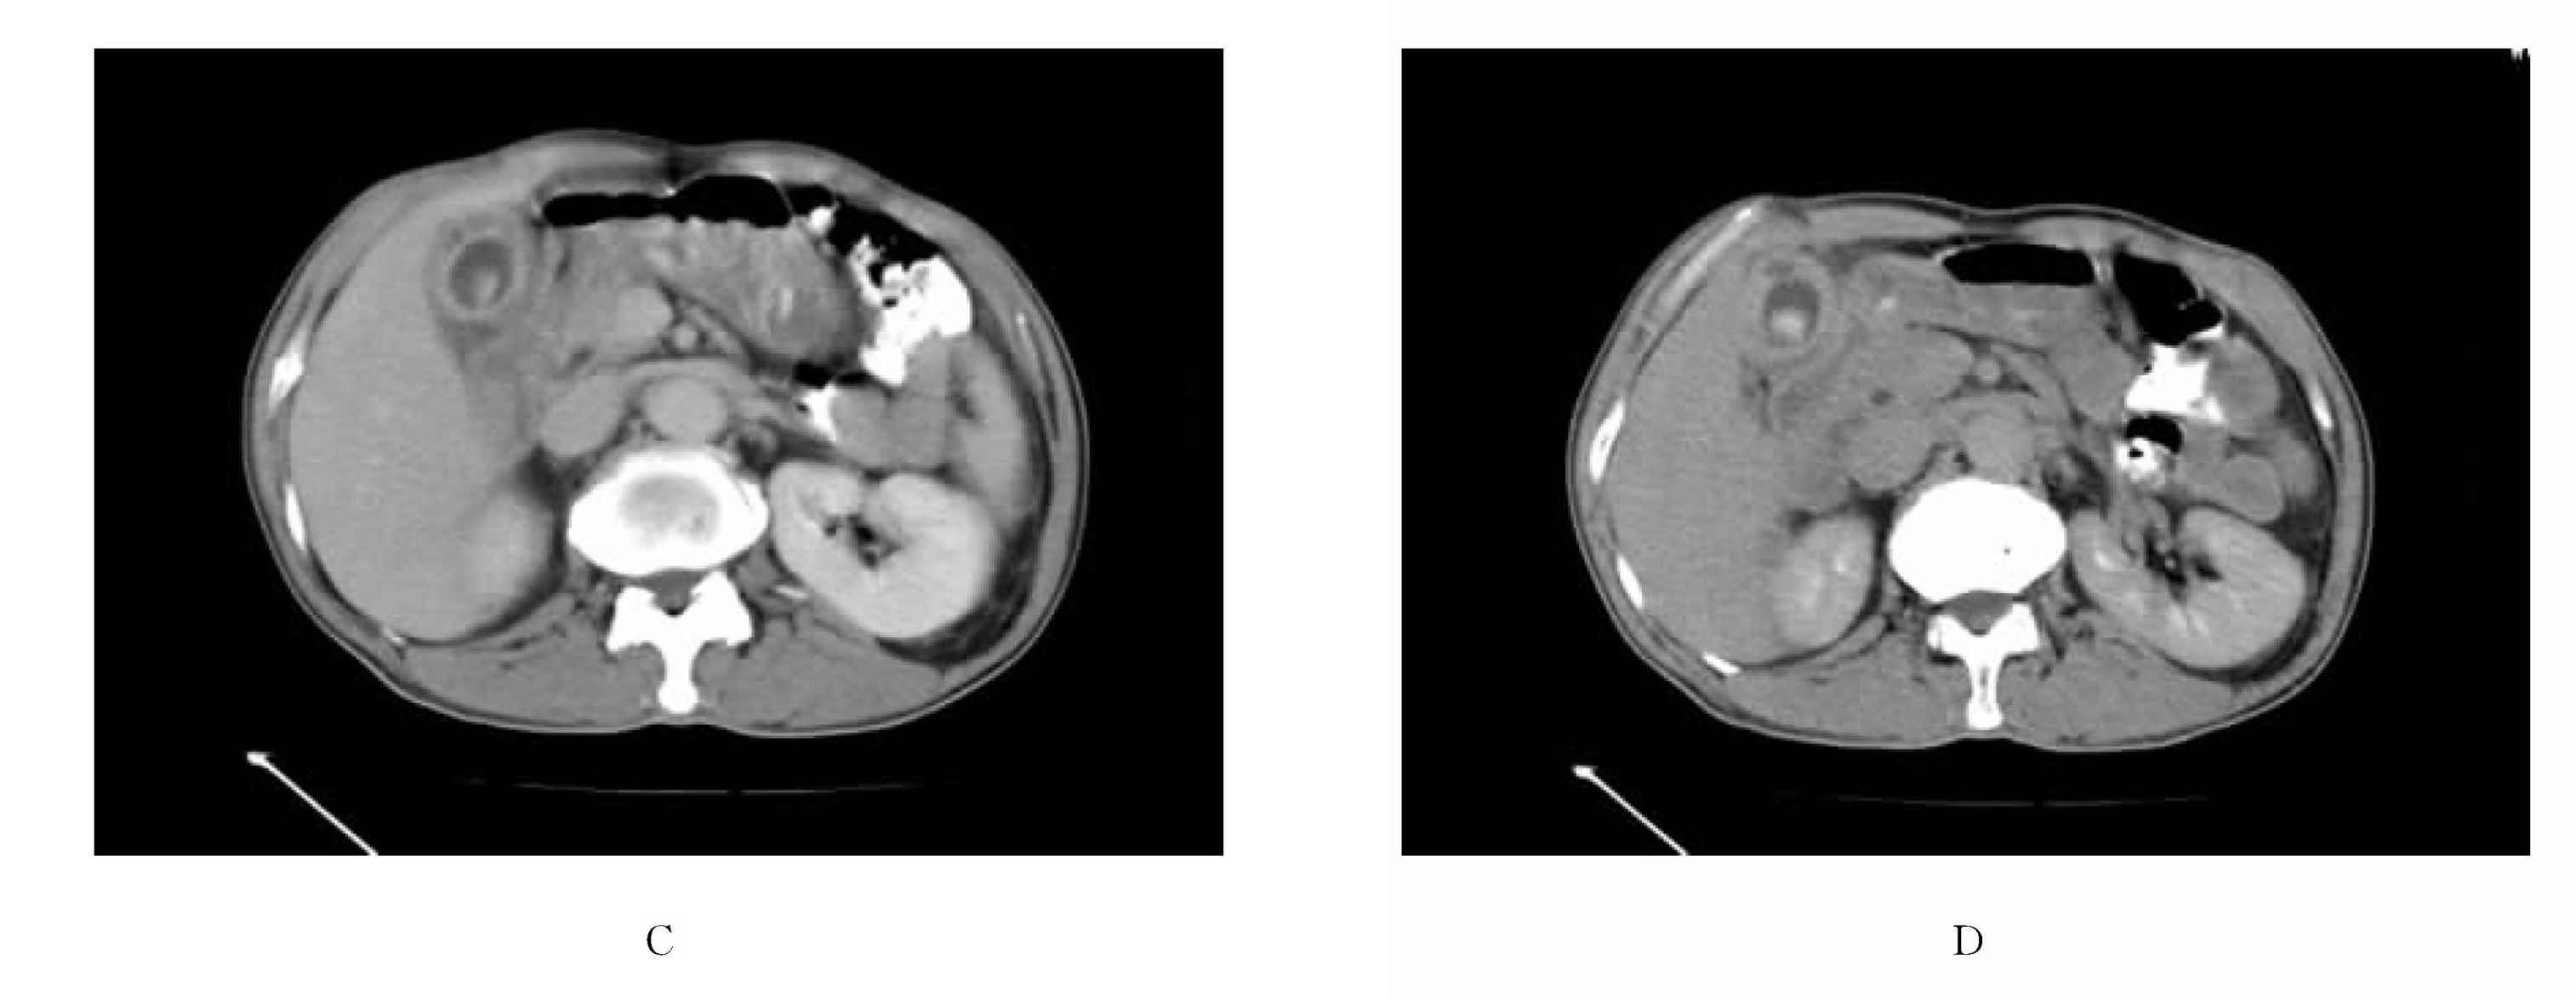
\includegraphics[width=.7\textwidth,height=\textheight,keepaspectratio]{./images/Image00299.jpg}
 \captionsetup{justification=centering}
 \caption{肝门区胆管癌\\{\small A、B为动脉期上下连续层面,C、D为门静脉期上下连续层面。B、D可见局部管壁不规则增厚,且均有强化;A、C可见近端胆管略扩张}}
 \label{fig12-8}
  \end{figure} 

其他征象:肝内胆管扩张,肝叶萎缩,肝脏、胆囊受侵,肝动脉、门静脉闭塞,肝内、腹腔、肝门区淋巴结转移等。

国外还有学者将肝门型胆管癌分为3类,即浸润型、外生型和腔内型,并认为浸润型动脉期强化率大;外生型在门脉期显示明显强化;而腔内型较少强化。还有学者报道肝门区胆管癌的增强扫描相对于肝脏密度呈高、低、高的强化趋势。75%门脉期和延迟期显示清楚,近70%出现延迟强化(延迟5~15分钟强化),15分钟后密度逐渐降低。

2.远段胆管癌

主要CT表现为胆道低位梗阻征象,肝内胆管及肝门区肝外胆管扩张,胆囊一般无扩大;扩张的胆总管突然狭窄和中断。薄层扫描可显示胆管内软组织结节或管壁的不规则增厚,以及梗阻以上胆管偏心性增厚等。增强扫描病灶有延迟强化表现。

国内有学者主张将肿瘤直径≤2cm的胆总管癌称为小胆总管癌。小胆总管癌的诊断关键是能够显示病灶,肿瘤在动脉期和门脉期明显强化,或者显示胆总管壁增厚超过2mm的强化,是诊断小胆总管癌的要点。同时,除肝内、外胆管扩张和胆囊增大外,胰管常不扩张。胆总管炎症时,其壁亦可呈环状强化,但其壁厚不超过2mm是鉴别的要点。

\subsection{壶腹区癌}

壶腹区癌又称为胆胰管十二指肠连接区癌。该区包括胆总管下端、胰管远端与十二指肠乳头及其周围2cm范围,故壶腹区癌是胰头癌、胆总管下端癌、Vater壶腹癌、十二指肠乳头癌的总称。还有人将Vater壶腹癌分为壶腹内型和十二指肠乳头型,即把十二指肠乳头癌归为Vater壶腹癌。

\textbf{【临床表现】}
主要表现为黄疸、腹胀,部分有发热、腹痛、体重减轻等。

\textbf{【CT表现】}

\subsubsection{常见表现}

1.胰头癌;多有胰头及钩突的增大,易伴体、尾萎缩。增强扫描病灶呈低密度区或不均匀低密度区。

2.胆总管下端癌及Vater壶腹癌:主要表现为胆管下端突然截断或管壁不规则、偏心性增厚,而肿块或结节可不能明确显示。增强扫描多有强化。

3.十二指肠乳头癌:由碘对比剂充盈良好的十二指肠可显示十二指肠乳头癌的软组织结节。

此外,壶腹区癌可靠的间接征象是胰、胆管高度扩张(出现双管征)和胆总管下端突然截断。但胆总管下端癌与Vater壶腹癌的鉴别有局限性,如壶腹区癌肿形成巨大肿块和周围浸润区别其来源更是困难的。

\subsubsection{壶腹区小癌灶}

所谓小壶腹区癌尚无统一影像学标准,多倾向于肿块≤3cm。国内学者报道有以下CT特点。

1.胰头及钩突癌:平扫、增强扫描为低密度区或不均匀低密度区,边缘模糊。可能是因癌巢间有大量纤维组织增生、血管少,周围胰腺组织呈炎性反应所致。

2.Vater壶腹癌:平扫可见边缘清楚的软组织结节;增强扫描有明显强化。是因其恶性程度低,癌组织接近正常组织,血供相对丰富所致。

3.胆总管癌:除管腔内结节、管壁局限性增厚外,常合并胆总管炎性增厚。CT可见结节及管壁增厚,并多有均匀强化(详见胆管癌部分所述)。

\textbf{【鉴别诊断】}

1.炎症:壶腹区肿瘤尤其是小肿瘤与炎症鉴别常较困难。主要鉴别点为:①炎症性胰头增大边缘无分叶和结节;肿瘤所致胰头增大常有分叶和结节表现。②胰头炎症边缘模糊,与周围结构界限不清;胰头癌边缘相对清楚。③胰头炎症密度均匀,胰腺实质内的小叶及其间的脂肪结构消失,或在均匀密度的基础上有散在分布的、小点状的水样低密度灶;胰头癌多表现为局限性、边缘模糊的低密度灶。④胆管的炎症管壁增厚与周围胰腺有分界;胆管癌则管壁与胰腺组织融合。胆管炎症患者可有胆道积气;而肿瘤一般则无。炎性(包括胰腺炎)胆管狭窄多为渐进性,且壁厚多<2mm,光滑规则;而肿瘤则为胆管突然截断及不规则管壁增厚,厚度多>2mm。但是,胆总管下端逐渐狭窄亦不能完全排除肿瘤可能,瘤细胞沿管壁浸润性生长或肿瘤合并炎症,均可出现此表现。

2.混合性胆管结石:密度如与软组织相似,需与壶腹区癌鉴别。①前者可见与胆管壁间有一圈或新月形近水样(胆汁)低密度环绕(即晕环征或新月征),增强扫描无强化;后者则见胆管突然截断,有强化。②胆总管结石的黄疸和临床症状可呈间断性;而肿瘤一般呈进行性加重。

3.十二指肠乳头水肿:可表现为十二指肠充盈缺损而与壶腹癌很难鉴别。但水肿边缘较光整,无进行性黄疸,治疗复查可明显缩小或消失。

\subsection{梗阻性黄疸的CT诊断}

\subsubsection{肝门区胆管梗阻}

常见病因:多见于恶性肿瘤。①胆管癌;②胆囊癌;③肝细胞癌;④肝门淋巴结转移癌;⑤肝总管结石。

\textbf{【CT表现】}
高位胆道梗阻,肝内胆管扩张。一般结石所致胆管扩张程度比肿瘤轻,恶性肿瘤可见局部软组织肿块。

\subsubsection{肝总管梗阻}

常见病因:①胆管癌:最常见,常造成胆管明显扩张。梗阻部位变化截然,肿瘤常较小而不易显示。薄层扫描有利于病灶显示。②结石:少见,胆管扩张程度较轻,可见结石影像。③胆囊癌:晚期直接侵犯或淋巴结转移压迫浸润肝总管。④淋巴结转移癌:压迫并可浸润肝总管。此外,也可由炎性狭窄所致。

\textbf{【CT表现】}
肝内胆管及肝门区肝外胆管扩张,一般胆囊无扩大,胆囊管无扩张。肿瘤、结石和炎症有相应的表现。

\subsubsection{胆总管梗阻}

常见病因:①胆管癌:胆管扩张较著,变化截然,胆管横断面从圆形扩张变为不规则形,薄层扫描可见管壁的不规则或偏心性增厚。②胰头癌:常合并胰管扩张,可见胰头部肿块。③胆总管结石:胆管扩张程度较轻,常可见肝外胆管逐渐变细(此表现亦可见于胆总管的炎性狭窄),于最下层面可见结石。④淋巴结转移癌:压迫并可浸润胆总管。此外,也可由炎性狭窄所致。

\textbf{【CT表现】}
较广泛的胆管扩张、胆囊扩大(但胆囊有慢性炎症时可不扩大)、胆囊管扩张。肿瘤、结石和炎症有相应的表现。

\subsubsection{壶腹部梗阻}

常见病因:①壶腹区癌:可合并胰管扩张,但常不能明确的显示胆总管及其周围肿块。②结石:胆管扩张程度常较轻,亦可见肝外胆管逐渐变细。此外,也可由炎性狭窄所致。

\textbf{【CT表现】}
低位胆道梗阻,全部胆道系统均显示扩张,胰管也扩张。特点是梗阻部位低,钩突内可见扩张的胆总管。

\subsubsection{肝内胆管扩张程度的判断}

1.依胆管扩张范围分为:①轻度:仅肝门附近胆管扩张;②中度:既有肝门,又有外围胆管扩张;③重度:肝门及外周胆管均明显扩张。

2.依胆管扩张宽度分为:①轻度:肝内胆管Ⅰ~Ⅱ级分支直径达0.5cm;②中度:直径0.6~0.8cm;③重度:直径0.9cm以上。

\protect\hypertarget{text00020.html}{}{}

